\AtBeginDocument{%
\begingroup\pagestyle{empty}\raggedright\parindent0pt
%\vspace*{-90pt}
%\begin{changemargin}{-60pt}{-60pt}
%{\fontsize{70}{1000}\Cobraarisca{
%\mbox{\noindent\rlap{\enspace C C C C C}{C C C C C C}}
%\mbox{\noindent\rlap{\enspace C C C C C}{C C C C C C}}
%\mbox{\noindent\rlap{\enspace C C C C C}{C C C C C C}}
%\mbox{\noindent\rlap{\enspace C C C C C}{C C C C C C}}
%\vspace{-18pt}{
%\mbox{\noindent\rlap{\enspace C C C C C}{C C C C C C}}}
%\mbox{\noindent\rlap{\enspace C C C l C}{C C C C C C}}
%\mbox{\noindent\rlap{\enspace C C C C C}{C C C C C C}}
%\mbox{\noindent\rlap{\enspace C C C C C}{C C C C C C}} \enlargethispage{\textheight}
%\mbox{\noindent\rlap{\enspace C C C C C}{C C C C C C}}
%\mbox{\noindent\rlap{\enspace C C C C C}{C C C C C C}}
%\mbox{\noindent\rlap{\enspace C C C C C}{C C C C C C}}
%}}
%\end{changemargin}
\begin{flushright}
\begin{vplace}[30]
``(\ldots{}) Um homem toma posse de si mesmo por meio de lampejos, e muitas vezes quando toma posse de si não se encontra nem se alcança. (\ldots{})''

\vspace*{0.2cm}

A. Artaud,
\textit{Carta para Jacques Rivière} em 25 de maio de 1924
\end{vplace}
\end{flushright}

%\LARGE{\autor}
%\vfill
\clearpage

%% Créditos ------------------------------------------------------
\raggedright

%{\Formular{\normalsize{N-1 edições \hspace{4.6cm} Coleção
%
%\vspace*{-5mm}
%
%\& Hedra \hspace{5cm} Lampejos}}}

%\bigskip
\linhalayout{Coleção Lampejos}{}
{\tiny{©n-1 edições 2019 / Hedra}}

\vspace*{0.5cm}

\linhalayout{\emph{A contracultura, entre a curtição e o experimental}}{}
\linhalayout{\emph{Celso Favaretto}}{}
{\tiny{©n-1 edições 2019}}

\vspace*{1cm}

\linha{tradução©}{\copyrighttraducao}
\linhalayout{coordenação editorial}{Peter Pál Pelbart e Ricardo Muniz Fernandes}
\linhalayout{direção de arte}{Ricardo Muniz Fernandes}
\linhalayout{preparação}{Tiago Ferro}
\linhalayout{projeto da coleção/capa}{Lucas Kröeff}
\linhalayout{ilustração/alfabeto}{Waldomiro Mugrelise}
\linha{coedição}{\coedicao}
\linha{assistência editorial}{\assistencia}
\linha{ISBN}{\ISBN}\smallskip
\linha{revisão}{\revisao}
\linha{preparação}{\preparacao}
\linha{iconografia}{\iconografia}
\linha{imagem da capa}{\imagemcapa}\smallskip
\begingroup\tiny
%\ifdef{\conselho}{\conselho}{\relax}
\par\endgroup\bigskip
%
\begingroup \tiny
%
\textit{Grafia atualizada segundo o Acordo Ortográfico da Língua\\
Portuguesa de 1990, em vigor no Brasil desde 2009.}\\
%

\begin{vplace}[30]
\vfill\textit{Direitos reservados em l\'ingua\\ portuguesa somente para o Brasil}\\\medskip
%%
\textsc{n-1 edições}\\
R.~Frei Caneca, 322 (cj 52)\\
São Paulo-\textsc{sp}, Brasil\\
\end{vplace}

\endgroup

%{\scriptsize\fakereceipt{
%A CONTRACULTURA,\\
%ENTRE A CURTIÇÃO\\
%E O EXPERIMENTAL

%\vspace{1cm}

%CELSO FAVARETTO

%\vspace{2cm}

%DESENHOS\\
%\vspace{0.5cm}
%WALDOMIRO\\
%\hspace{1.7cm}MUGRELISE\\

%\vspace{1cm}

%COLEÇÃO LAMPEJOS

%\vspace{0.5cm}

%PRIMEIRA EDIÇÃO

%\vspace{0.5cm}

%COPYRIGHT: HEDRA \& N-1\\
%EDIÇÃO: RICARDO MUNIZ\\
%PROJETO DA COLEÇÃO: L.KRÖEFF\\
%TIRAGEM: 1\textsuperscript{A TIRAGEM} 300UN\\
%ISBN: XXXXXXXXXXXXXXXXXXXXX\\

%\vspace{1cm}

%PUBLICADO POR\\
%HEDRA \& N-1\\
%SÃO PAULO, 2019\\
%IMPRESSA SOB DEMANDA\\

%\vspace{0.5cm}

%RUA FRADIQUE COUTINHO, 1139\\
%05416-011 SÃO PAULO, SP BRASIL
%}}
\pagebreak

%\vspace*{-80pt}
\begin{changemargin}{-85pt}{-60pt}
{\Formular{

\mbox{\textbf{Celso Favaretto} \hspace{0.6cm}\textbf{Celso Favaretto} \hspace{0.6cm}\textbf{Celso Favaretto} \hspace{0.6cm}\textbf{Celso Favaretto}}\vspace*{-3pt}
\mbox{A contracultura, \hspace{0.7cm}A contracultura, \hspace{0.7cm}A contracultura, \hspace{0.7cm}A contracultura,}\vspace*{-3pt}
\mbox{entre a curtição \hspace{0.7cm}entre a curtição \hspace{0.75cm}entre a curtição \hspace{0.75cm}entre a curtição}\vspace*{-3pt}
\mbox{e o experimental \hspace{0.57cm}e o experimental \hspace{0.62cm}e o experimental \hspace{0.62cm}e o experimental}
}}
\end{changemargin}
%% Front ---------------------------------------------------------
% Titulo


%{\LARGE{\autor} \par}%\vspace{1.5ex}}
%\vspace{6cm} %9.3cm
%\ifdef{\organizador}{{\small {\organizador} (\textit{organização})} \par}{}
%\ifdef{\introdutor}{{\small {\introdutor} (\textit{prefácio})} \par}{}
%\ifdef{\tradutor}{{\small {\tradutor} (\textit{tradução})}\par}{}\vspace{8.5mm}

%{{\footnotesize{} \ifdef{\numeroedicao}{\numeroedicao}{2}ª edição} \par}
%logos
\vfill
%\normalsize
%\ifdef{\logo}{\IfFileExists{\logo}{\hfill\includegraphics[width=3cm]{\logo}\hfill\logoum{}\\ São Paulo\_\the\year}}{\logoum\break{} São Paulo\_\the\year}
%\includegraphics[width=.4\textwidth,trim=0 0 25 0]{logo.jpg}\\\smallskip
\par\clearpage\endgroup
% Resumo -------------------------------------------------------
\begingroup \footnotesize \parindent0pt \parskip 5pt \thispagestyle{empty} \vspace{1cm}%\textheight}\mbox{} \vfill
\movetoevenpage
\raggedright
{\Formular{\textit{O livro como imagem do mundo é de toda maneira uma ideia insípida. Na verdade não basta dizer Viva o múltiplo, grito de resto difícil de emitir. Nenhuma habilidade tipográfica, lexical ou mesmo sintática será suficiente para fazê-lo ouvir. É preciso fazer o múltiplo, não acrescentando sempre uma dimensão superior, mas, ao contrário, da maneira mais simples, com força de sobriedade, no nível das dimensões de que se dispõe, sempre n-1 (é somente assim que o uno faz parte do múltiplo, estando sempre subtraído dele). Subtrair o único da multiplicidade a ser constituída; escrever a n-1.}}}

\vspace*{4pt}

{\Formular{\textit{Gilles Deleuze e Félix Guattari}}}
\movetooddpage
\baselineskip=.92\baselineskip
\IfFileExists{PRETAS.tex}{\raggedright

{\Formular{\textbf{CELSO FAVARETTO}}} {\Formular{\textit{é pesquisador. Licenciado em Filosofia. É Mestre e Doutor em Filosofia, concentração em estética, pela Universidade de São Paulo. Foi professor de Filosofia e Estética em diversos colégios e universidades, como a PUC-SP. Desde 1985, é professor na Faculdade de Educação da USP, no curso de Licenciatura em Filosofia e no programa de Pós-Graduação, sendo também professor-orientador na área de Estética do programa de Filosofia da Faculdade de Filosofia, Letras e Ciências Humanas da mesma universidade.}

\textit{Publicou os livros “Tropicália, alegoria alegria” (São Paulo, Kairós, 1979; 3. ed. rev., São Paulo, Ateliê Editorial, 2000) e “A invenção de Hélio Oiticica” (São Paulo, Editora da Universidade de São Paulo, 1992; 2. ed. rev., 2000), além de ensaios e artigos em livros coletivos, jornais e revistas. O livro “Tropicália, alegoria alegria”, esgotado nas livrarias, é considerado um dos mais completos trabalhos sobre Tropicalismo. Em 2001, participou do seminário “Da bossa nova à tropicália”, realizado pelo Cesap/Faperj na Universidade Cândido Mendes.}}}




}{% 
\ifdef{\resumo}{\resumo\par}{}
\ifdef{\sobreobra}{\sobreobra}{}
\ifdef{\sobreautor}{\mbox{}\vspace{4pt}\newline\sobreautor}{}
\ifdef{\sobretradutor}{\newline\sobretradutor}{\relax}
\ifdef{\sobreorganizador}{\vspace{4pt}\newline\sobreorganizador}{\relax}\par}
\thispagestyle{empty} \endgroup
\ifdefvoid{\sobreautor}{}{\pagebreak\ifodd\thepage\paginabranca\fi}
% Sumário -------------------------------------------------------

%\sumario{}
%\IfFileExists{INTRO.tex}{\include{INTRO}}

%\IfFileExists{TEXTO.tex}{\mbox{}\part{A contracultura, entre a curtição e o experimental}

\lipsum

Nam dui ligula,\footnote{Lorem ipsum dolor sit amet, consectetur adipiscing elit. In
ultrices neque id venenatis tincidunt. Nam non nisl cursus,
faucibus dolor in, bibendum arcu. Praesent consectetur sem
erat, ac consequat tellus laoreet sed. Donec consectetur tris-
tique magna ornare aliquam. Sed maximus maximus vestib-
ulum. Fusce ac lacus et ex finibus finibus ac condimentum
lorem. Curabitur dictum at ligula tincidunt vestibulum.} fringilla a, euismod sodales, sollicitudin
vel, wisi. Morbi auctor lorem non justo. Nam lacus libero,
pretium at, lobortis vitae, ultricies et, tellus. Donec aliquet,
tortor sed accumsan bibendum, erat ligula aliquet magna,
vitae ornare odio metus a mi. Morbi ac orci et nisl hendrerit
mollis. Suspendisse ut massa. Cras nec ante. Pellentesque
a nulla. Cum sociis natoque penatibus et magnis dis par-
turient montes, nascetur ridiculus mus. Aliquam tincidunt
urna. Nulla ullamcorper vestibulum turpis. Pellentesque
cursus luctus mauris

\pagebreak

\thispagestyle{empty}

\vspace*{-80pt}

{\large\fakereceipt{

\noindent\mbox{\noindent\hspace*{-175pt}CELSO FAVARETTO \mbox{  }\mbox{  }CELSO FAVARETTO \mbox{  }\mbox{  }CELSO FAVARETTO\\}
\mbox{\hspace*{-175pt}A CONTRACULTURA, \mbox{  }A CONTRACULTURA, \mbox{  }A CONTRACULTURA,\\}
\mbox{\hspace*{-175pt}ENTRE A CURTIÇÃO \mbox{  }ENTRE A CURTIÇÃO \mbox{  }ENTRE A CURTIÇÃO\\}
\mbox{\hspace*{-175pt}E O EXPERIMENTAL \mbox{  }E O EXPERIMENTAL \mbox{  }E O EXPERIMENTAL}

\noindent\mbox{\noindent\hspace*{-40pt}CELSO FAVARETTO \mbox{  }\mbox{  }CELSO FAVARETTO \mbox{  }\mbox{  }CELSO FAVARETTO\\}
\mbox{\hspace*{-40pt}A CONTRACULTURA, \mbox{  }A CONTRACULTURA, \mbox{  }A CONTRACULTURA,\\}
\mbox{\hspace*{-40pt}ENTRE A CURTIÇÃO \mbox{  }ENTRE A CURTIÇÃO \mbox{  }ENTRE A CURTIÇÃO\\}
\mbox{\hspace*{-40pt}E O EXPERIMENTAL \mbox{  }E O EXPERIMENTAL \mbox{  }E O EXPERIMENTAL}

\noindent\mbox{\noindent\hspace*{-140pt}CELSO FAVARETTO \mbox{  }\mbox{  }CELSO FAVARETTO \mbox{  }\mbox{  }CELSO FAVARETTO\\}
\mbox{\hspace*{-140pt}A CONTRACULTURA, \mbox{  }A CONTRACULTURA, \mbox{  }A CONTRACULTURA,\\}
\mbox{\hspace*{-140pt}ENTRE A CURTIÇÃO \mbox{  }ENTRE A CURTIÇÃO \mbox{  }ENTRE A CURTIÇÃO\\}
\mbox{\hspace*{-140pt}E O EXPERIMENTAL \mbox{  }E O EXPERIMENTAL \mbox{  }E O EXPERIMENTAL}

\noindent\mbox{\noindent\hspace*{-160pt}CELSO FAVARETTO \mbox{  }\mbox{  }CELSO FAVARETTO \mbox{  }\mbox{  }CELSO FAVARETTO\\}
\mbox{\hspace*{-160pt}A CONTRACULTURA, \mbox{  }A CONTRACULTURA, \mbox{  }A CONTRACULTURA,\\}
\mbox{\hspace*{-160pt}ENTRE A CURTIÇÃO \mbox{  }ENTRE A CURTIÇÃO \mbox{  }ENTRE A CURTIÇÃO\\}
\mbox{\hspace*{-160pt}E O EXPERIMENTAL \mbox{  }E O EXPERIMENTAL \mbox{  }E O EXPERIMENTAL}

\noindent\mbox{\noindent\hspace*{-180pt}CELSO FAVARETTO \mbox{  }\mbox{  }CELSO FAVARETTO \mbox{  }\mbox{  }CELSO FAVARETTO\\}
\mbox{\hspace*{-180pt}A CONTRACULTURA, \mbox{  }A CONTRACULTURA, \mbox{  }A CONTRACULTURA,\\}
\mbox{\hspace*{-180pt}ENTRE A CURTIÇÃO \mbox{  }ENTRE A CURTIÇÃO \mbox{  }ENTRE A CURTIÇÃO\\}
\mbox{\hspace*{-180pt}E O EXPERIMENTAL \mbox{  }E O EXPERIMENTAL \mbox{  }E O EXPERIMENTAL}

\noindent\mbox{\noindent\hspace*{-38pt}CELSO FAVARETTO \mbox{  }\mbox{  }CELSO FAVARETTO \mbox{  }\mbox{  }CELSO FAVARETTO\\}
\mbox{\hspace*{-38pt}A CONTRACULTURA, \mbox{  }A CONTRACULTURA, \mbox{  }A CONTRACULTURA,\\}
\mbox{\hspace*{-38pt}ENTRE A CURTIÇÃO \mbox{  }ENTRE A CURTIÇÃO \mbox{  }ENTRE A CURTIÇÃO\\}
\mbox{\hspace*{-38pt}E O EXPERIMENTAL \mbox{  }E O EXPERIMENTAL \mbox{  }E O EXPERIMENTAL}

\noindent\mbox{\noindent\hspace*{-140pt}CELSO FAVARETTO \mbox{  }\mbox{  }CELSO FAVARETTO \mbox{  }\mbox{  }CELSO FAVARETTO\\} \enlargethispage{\textheight}
\mbox{\hspace*{-140pt}A CONTRACULTURA, \mbox{  }A CONTRACULTURA, \mbox{  }A CONTRACULTURA,\\}
\mbox{\hspace*{-140pt}ENTRE A CURTIÇÃO \mbox{  }ENTRE A CURTIÇÃO \mbox{  }ENTRE A CURTIÇÃO\\}
\mbox{\hspace*{-140pt}E O EXPERIMENTAL \mbox{  }E O EXPERIMENTAL \mbox{  }E O EXPERIMENTAL}

\noindent\mbox{\noindent\hspace*{-160pt}CELSO FAVARETTO \mbox{  }\mbox{  }CELSO FAVARETTO \mbox{  }\mbox{  }CELSO FAVARETTO\\} 
\mbox{\hspace*{-160pt}A CONTRACULTURA, \mbox{  }A CONTRACULTURA, \mbox{  }A CONTRACULTURA,}
}}

%\vspace*{-65pt}
%{\large\fakereceipt{
%\noindent CELSO FAVARETTO CELSO FAVARETTO\\
%A CONTRACULTURA, A CONTRACULTURA,\\
%ENTRE A CURTIÇÃO ENTRE A CURTIÇÃO\\
%E O EXPERIMENTAL E O EXPERIMENTAL}} 


}
%\part[{{\def\break{}\titulo}}]{\titulo}
} % fim do AtBeginDocument

% Finais -------------------------------------------------------
\AtEndDocument{%
  %\publicidade
%
\pagebreak\ifodd\thepage\paginabranca\fi
{\raggedright

\includegraphics[width=.4\textwidth]{./logos.jpg}{}
}

\vspace*{5cm}

{\centering
\hspace*{0.5pt}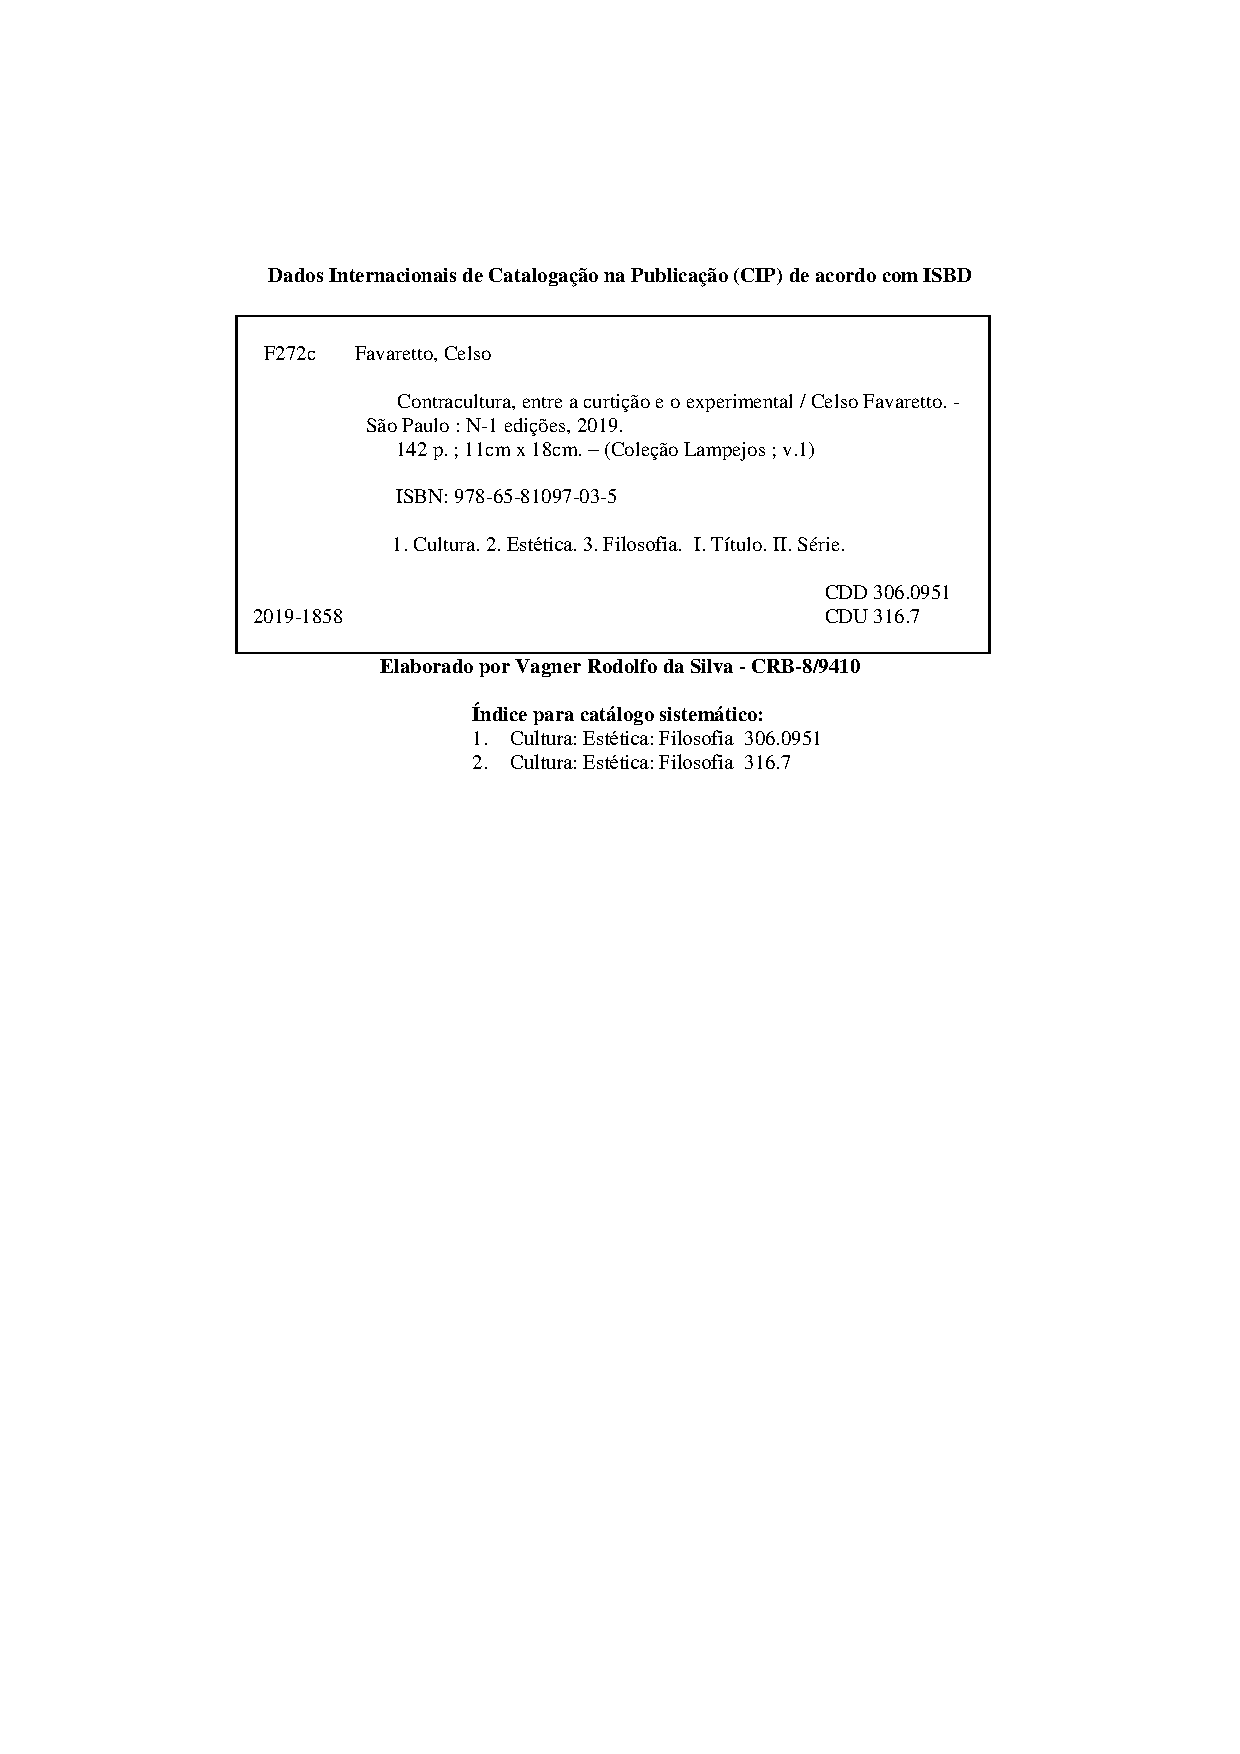
\includegraphics[width=1\textwidth]{./ficha.pdf}{}}
}%
%\mbox{}\vfill\small\thispagestyle{empty}
%\begin{center}
%\begin{minipage}{.8\textwidth}
%\centering\tiny\noindent{}Adverte-se aos curiosos que se imprimiu este livro \ifdef{\grafica}{na %gráfica \grafica}{em nossas oficinas}, 
%em \today \ifdef{\papelmiolo}{em papel \papelmiolo}, em tipologia \tipopadrao{}, com diversos %sofwares livres, 
%entre eles, Lua\LaTeX, git \& ruby. \ifdef{\RevisionInfo{}}{\par(v.\,\RevisionInfo)}{}\par \begin{%center}\normalsize\adforn{64}\end{center}
%\end{minipage}
%\end{center}
%}
